\documentclass{ctexart}
\textheight 23.5cm \textwidth 15.8cm
\topmargin -1.5cm \oddsidemargin 0.3cm \evensidemargin -0.3cm

\usepackage{verbatim}
\usepackage{fancyhdr}
\usepackage{float}
\usepackage{graphicx}
\usepackage{amssymb}
\usepackage{amsmath}


\pagestyle{fancy}
\CTEXsetup[format = {\Large\bfseries\it}]{section}


\begin{document}

\section*{内容简介}
	\noindent 一、对函数
	\begin{equation}
		f(x) = e^x \qquad x\in[−5,\,5]
	\end{equation}
	对以下两种类型的样条函数:
	
	1.三次自然样条
	
	2.满足 $S'(0) = 1, S'(1) = e$ 的样条\\
	构造等距节点的三次样条插值函数,并计算如下误差
	\begin{equation}
		\max\limits_i\left\{\Big|f(x_{i − \frac{1}{2}}) − S(x_{i − \frac{1}{2}})\Big|,\quad\ i = 0, 1, \cdots, N\right\}
	\end{equation}
	这里 $x_{i − \frac{1}{2}}$ 为每个小区间的中点。对 $N = 10, 20, 40, 80$ 比较以上两组结点的结果。讨论结果。利用公式计算算法的收敛阶。\\
	
	\noindent 二、证明公式
	\begin{equation}
		\int_{t_i}^{t_i+1}S_i(x)dx = \dfrac{h_i}{2}(y_i + y_{i+1}) - \dfrac{h_i^3}{24}(z_i + z_{i+1})
	\end{equation}
	然后编写测试一个程序用于计算
	\begin{equation}
		\int_{t_0}^{t_n}S(x)dx
	\end{equation}
	
\section*{工作环境}
	程序所用语言: {\bf python}
	
	软件: {\bf JupyterLab}
	
	使用的包: {\bf numpy, matplotlib, bisect}

\section*{输出结果}

\begin{verbatim}
	N = 10
	Method (1) Error = 0.001241988377	
	Integrate[S1(x), {t_n, t_0}] = 1.718370963763
	
	Method (2) Error = 0.000005743028	
	Integrate[S2(x), {t_n, t_0}] = 1.718281589866
	
	
	N = 20
	Method (1) Error = 0.000310817170	Order = 1.998513566872
	Integrate[S1(x), {t_n, t_0}] = 1.718292992222
	
	Method (2) Error = 0.000000378048	Order = 3.925168949767
	Integrate[S2(x), {t_n, t_0}] = 1.718281813544
	
	
	N = 40
	Method (1) Error = 0.000077724487	Order = 1.999625103723
	Integrate[S1(x), {t_n, t_0}] = 1.718283225079
	
	Method (2) Error = 0.000000024249	Order = 3.962568282435
	Integrate[S2(x), {t_n, t_0}] = 1.718281827527
	
	
	N = 80
	Method (1) Error = 0.000019432392	Order = 1.999905714701
	Integrate[S1(x), {t_n, t_0}] = 1.718282003102
	
	Method (2) Error = 0.000000001535	Order = 3.981281459724
	Integrate[S2(x), {t_n, t_0}] = 1.718281828401
\end{verbatim}

\begin{figure}[H]
	\centering
	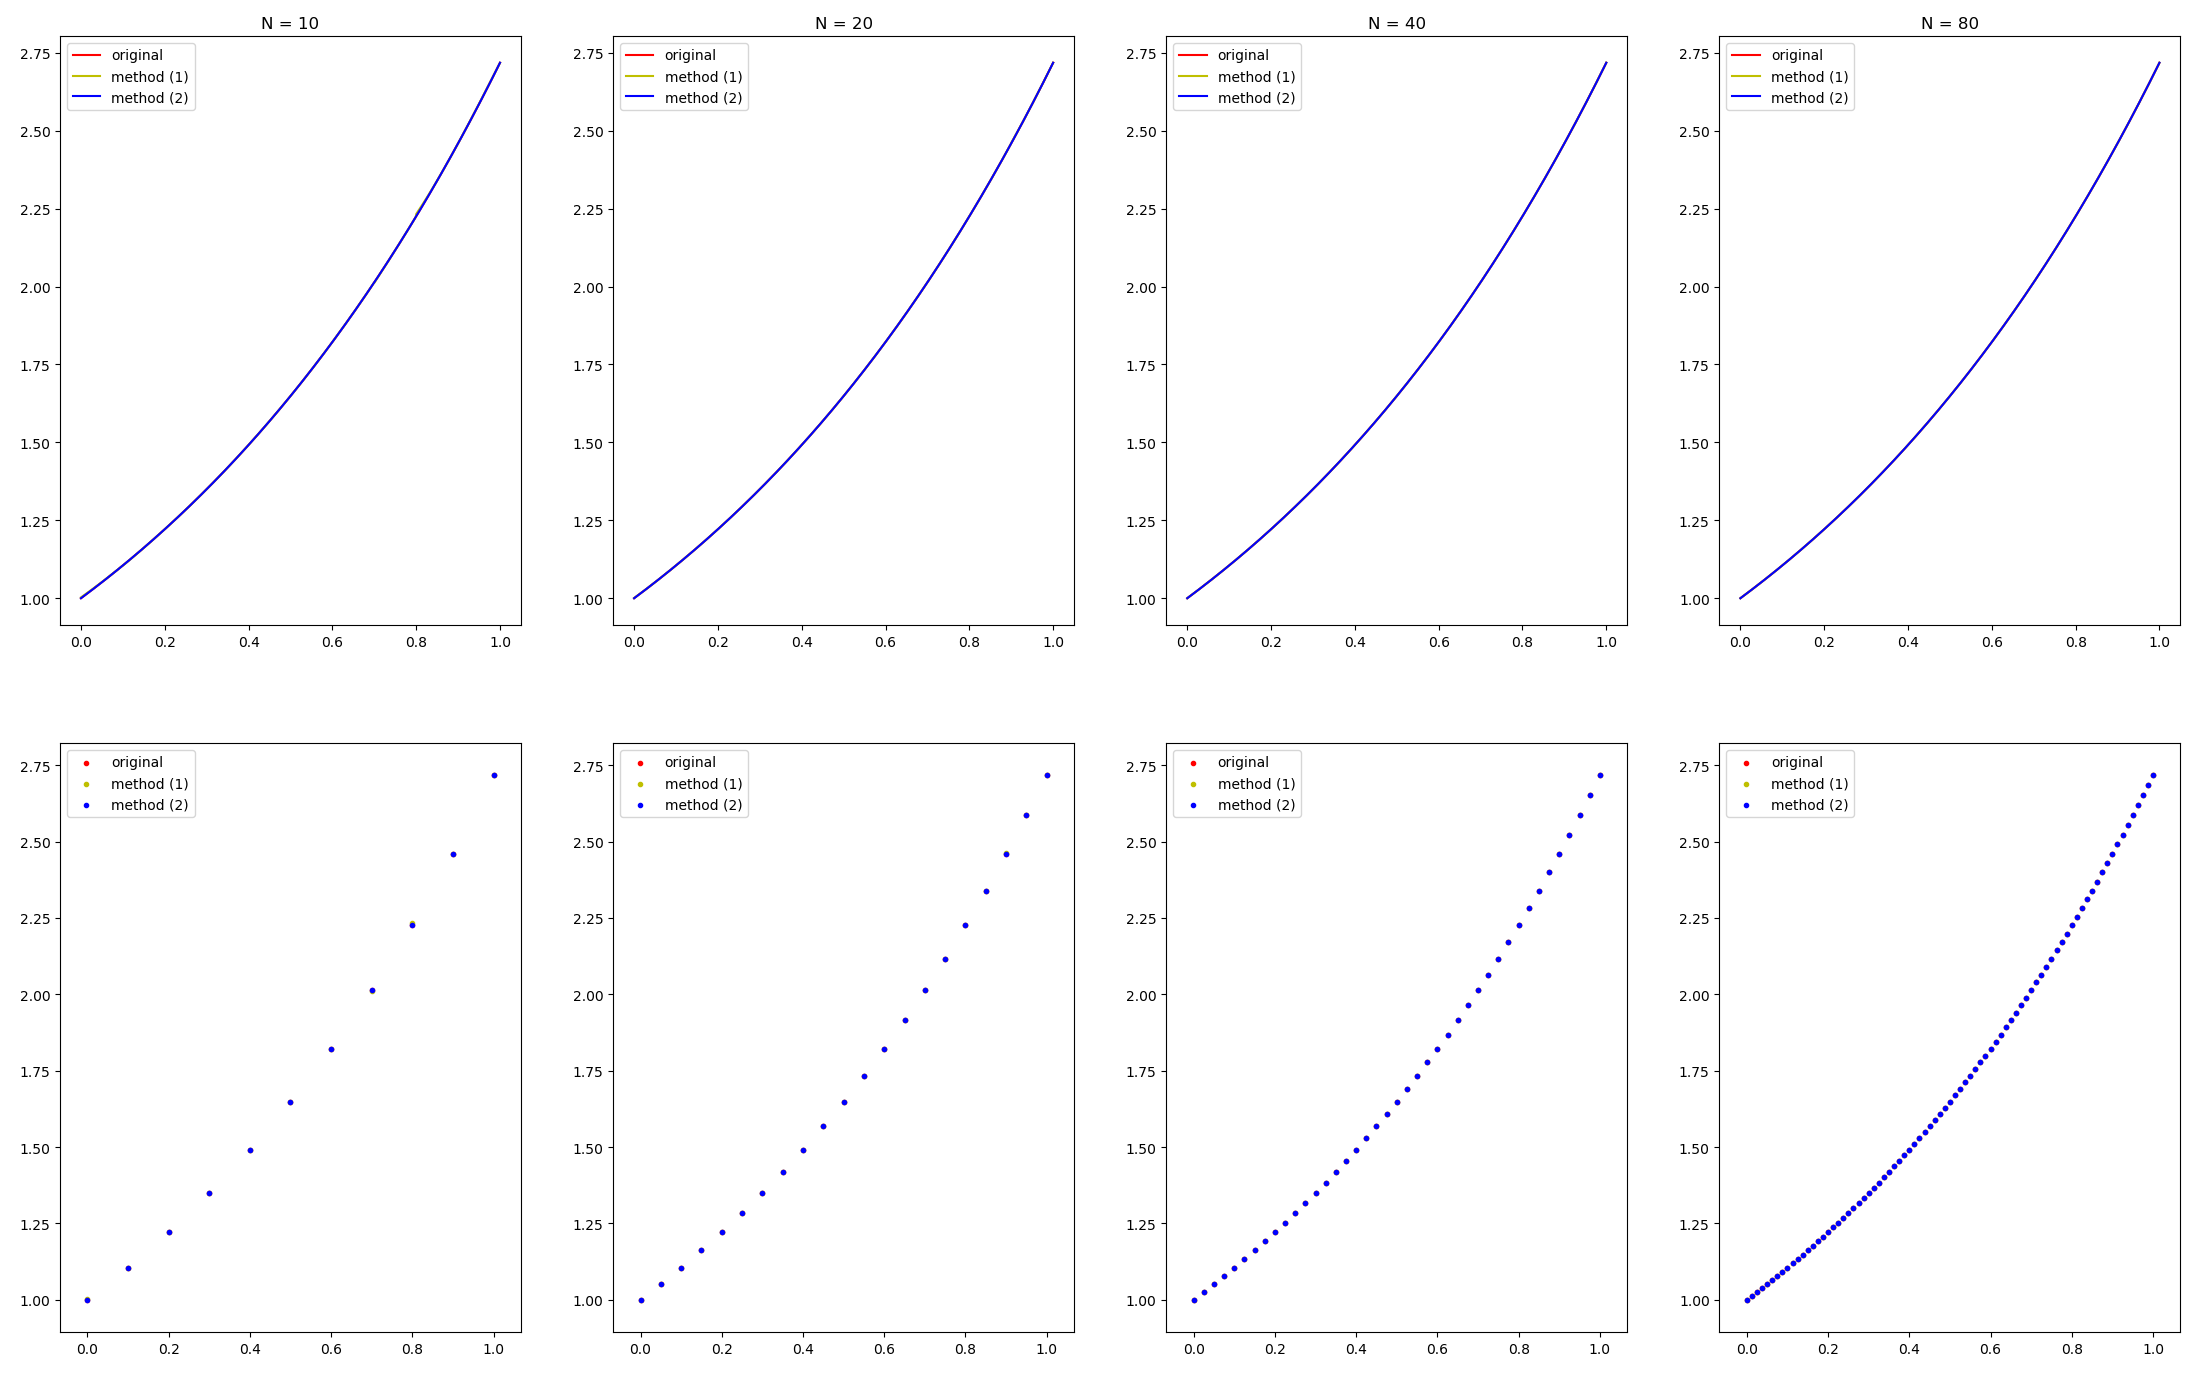
\includegraphics[width = 15cm, height = 8cm]{figure.png}
	\caption{两种不同的三次样条插值结果比较} \label{figure.label}
\end{figure}

\begin{table}[htb]
	\centering
	\bigskip
	\begin{small}
		\begin{tabular}{|c|cc|cc|}
			\hline
			n & Method (1) Error & order & Method (2) Error & order\\\hline
			10& 1.242E-03 & -- & 5.743E-06 & --\\
			20& 3.108E-04 & 1.9985 & 3.780E-07 & 3.9252 \\
			40& 7.772E-05 & 1.9996 & 2.425E-08 & 3.9626\\
			80& 1.943E-05 & 1.9999 & 1.535E-09 & 3.9813\\\hline
		\end{tabular}
	\end{small}
	\caption{\label{table.label} $L_\infty$ 范数意义下的精度检验} 
\end{table}

\section*{现象描述}
	\noindent 一、由图像可见三次样条函数在指定区间上拟合得非常好。而随着插值点数目的增加,样条与原函数的偏差也愈来愈小。计算出方法1自然样条的收敛阶约为2阶,而方法2的收敛阶约为4阶。
	
	\noindent 二、积分准确值应为 $1.718281828459$,由题中公式确实给出了较精确的计算结果。
\section*{公式证明}
	\begin{align*}
		&\int_{t_i}^{t_i+1}S_i(x)dx \\
		&= \int_{t_i}^{t_i+1}\left[\dfrac{z_i}{6h_i}(t_{i+1} - x)^3 + \dfrac{z_{i+1}}{6h_i}(x - t_i)^3 + (\dfrac{y_{i+1}}{h_i} - \dfrac{z_{i+1} h_i}{6})(x - t_i) + (\dfrac{y_i}{h_i} - \dfrac{z_i h_i}{6})(t_{i+1} - x)\right]dx \\
		&= \dfrac{z_i}{24h_i}(t_{i+1} - t_i)^4 + \dfrac{z_{i+1}}{24h_i}(t_{i+1} - t_i)^4 + (\dfrac{y_{i+1}}{2h_i} - \dfrac{z_{i+1} h_i}{12})(t_{i+1} - t_i)^2 + (\dfrac{y_i}{2h_i} - \dfrac{z_i h_i}{12})(t_{i+1} - t_i)^2\\
		&= \dfrac{h_i^3}{24}(z_i + z_{i+1}) + \dfrac{h_i}{2}(y_i + y_{i+1}) - \dfrac{h_i^3}{12}(z_i + z_{i+1})\\
		&= \dfrac{h_i}{2}(y_i + y_{i+1}) - \dfrac{h_i^3}{24}(z_i + z_{i+1})
	\end{align*}
	于是(二)中公式得证。
	
\section*{参考资料}
	\noindent [1] David R. Kincaid \& E. Ward Cheney. {\it Numerical Analysis: Mathematics of Scientific of Computing Third Edition}, Brooks/Cole, 2002.

\end{document}